\documentclass[notheorems, handout]{beamer}
\usetheme[numbers,totalnumbers,compress, nologo]{Statmod}
\usefonttheme[onlymath]{serif}
\setbeamertemplate{navigation symbols}{}

\usepackage[utf8]{inputenc}
\usepackage[T2A]{fontenc}
\usepackage[russian]{babel}

\usepackage{graphicx,subcaption,ragged2e}
\usepackage{tikz}
\usepackage{hhline}

\setbeamercolor{bluetext_color}{fg=blue}
\newcommand{\bluetext}[1]{{\usebeamercolor[fg]{bluetext_color}#1}}

\usetikzlibrary{shapes.geometric, arrows}
\tikzstyle{arrow} = [thick,->,>=stealth]

\newcommand{\bfxi}{\boldsymbol{\xi}}
\newtheorem{definition}{Определение}
\newtheorem{remark}{Замечание}

\title[Выбор параметров в MC-SSA]{Выбор параметров в методе Monte Carlo SSA}

\author{Потешкин Егор Павлович}

\institute[Санкт-Петербургский Государственный Университет]{%
	\small
	Санкт-Петербургский государственный университет\\
	Кафедра статистического моделирования}

\date{\\Процессы управления и устойчивость\\2 апреля 2024, Санкт-Петербург}

\subject{Talks}	

\input{letters_series_mathbb.tex}

\begin{document}
\begin{frame}[plain]
	\titlepage
	\note{Научный руководитель  к.ф.-м.н., доцент Голяндина\,Н.\,Э.,\\
		кафедра статистического моделирования}
\end{frame}

\begin{frame}{Введение}
	\begin{figure}
		\centering
		\includegraphics[width=0.9\textwidth]{images/ts.pdf}
	\end{figure}
	\bluetext{Вопрос}: это чистый шум или там есть сигнал?
\end{frame}

\begin{frame}{Постановка задачи}
	$\tX=(x_1,\ldots,x_N)$, $x_i\in \mathbb{R}$ "--- временной ряд.\medskip

	\bluetext{Дано}: $\tX=\tT + \tH + \tR$, где $\tT$ "--- тренд, $\tH$ "--- сезонность и $\tR$ "--- шум.\medskip

	\bluetext{Проблемы}:
	\begin{enumerate}
		\item Как выделить неслучайные компоненты?\medskip
		\item \underline{Как проверить наличие сигнала $\tS=\tT + \tH$?}
	\end{enumerate}

	\bluetext{Методы}:
	\begin{enumerate}
		\item Singular spectrum analysis\linebreak(SSA)~[Broomhead and King, 1986].\medskip
		\item \underline{Monte-Carlo SSA (MC-SSA)}~[Allen and Smith, 1996] проверяет $H_0:\tS=0$.
	\end{enumerate}
	\bluetext{Задача}: исследовать зависимость радикальности и мощности MC-SSA от параметра $L$.
\end{frame}

\begin{frame}{Обозначения и известные результаты: оператор вложения и ганкелизации}
	$\tX=(x_1,\ldots,x_N)$. Зафиксируем $L$ ($1<L<N$).\medskip

	\emph{Оператор вложения} $\cT_\text{SSA}$:
	\begin{equation*}
		\cT_{\text{SSA}}(\tX)=\bfX=\begin{pmatrix}
			x_1    & x_2     & \cdots & x_K     \\
			x_2    & x_3     & \cdots & x_{K+1} \\
			\vdots & \vdots  & \ddots & \vdots  \\
			x_L    & x_{L+1} & \cdots & x_N
		\end{pmatrix},
	\end{equation*}
	где $K=N-L+1$.\medskip

	\emph{Оператор ганкелизации} $\cH$ "--- усреднение матрицы по побочным диагоналям.
\end{frame}

\begin{frame}{Обозначения и известные результаты: SSA}
	\bluetext{Входные данные}: временной ряд $\tX=(x_1,\ldots,x_N)$.\\

	\bluetext{Параметр}: длина окна $L$.\\

	\bluetext{Результат}: $m$ восстановленных составляющих временного ряда.\\
	\begin{figure}
		\scalebox{0.5}{
			\begin{tikzpicture}[node distance=2cm]
				\node[draw, align=center, minimum width=8.5cm, minimum height=3.25cm](1){{\LARGE\textbf{Входные данные}: $\tX$} "---\\\LARGE временной ряд};
				\node[draw, align=center, minimum width=8.5cm, minimum height=3.25cm, below of=1, yshift=-2cm](2){{\LARGE Траекторная матрица}\\ \LARGE $\bf{X}=\cT_{\text{SSA}}(\tX)$};
				\node[draw, align=center, minimum width=8.5cm, minimum height=3.25cm, right of=2, xshift=10cm](3){\LARGE Сумма матриц\\ \LARGE единичного ранга\\ \LARGE$\bfX=\sum\limits_{j=1}^d\bfX_j$};
				\node[draw, align=center, minimum width=8.5cm, minimum height=3.25cm, below of=3, yshift=-2cm](4){\LARGE Сгруппированные\\ \LARGE матрицы\\ \LARGE$\bfX=\bfX_{I_1}+\ldots+\bfX_{I_m}$\\\LARGE$\bfX_{I_k}=\sum\limits_{i\in I_k}\bfX_i$};
				\node[draw, align=center, minimum width=8.5cm, minimum height=3.25cm, below of=2, yshift=-2cm](5){\LARGE\textbf{Результат}: SSA разложение\\\LARGE$\tX=\widetilde\tX_{I_1}+\ldots+\widetilde\tX_{I_m}$\\\LARGE$\widetilde\tX_{I_k}=\cT_\text{SSA}^{-1}\circ\cH(\bfX_{I_k})$};

				\draw[arrow](1)--node[anchor=west]{\large1. Вложение}(2);
				\draw[arrow](2)--node[anchor=south]{\large2. Разложение}(3);
				\draw[arrow](3)--node[anchor=west]{\large3. Группировка}(4);
				\draw[arrow](4)--node[anchor=south]{\large4. Восстановление}(5);
			\end{tikzpicture}}
		\caption{Алгоритм SSA}
	\end{figure}
\end{frame}

\begin{frame}{Обозначения и известные результаты: Toeplitz SSA}
	Модификации SSA отличаются только шагом разложения.\medskip

	Basic SSA: сингулярное разложение траекторной матрицы, универсальный метод.\medskip

	Toeplitz SSA: теплицево разложение траекторной матрицы, имеет преимущество для стационарных рядов:
	\begin{equation*}
		\bfX=\sum_{i=1}^L\sigma_i P_iQ_i^\rmT = \bfX_1+\ldots +\bfX_L,
	\end{equation*}
	где $Q_i=\bfX^\rmT P_i/\sigma_i$, $\sigma_i=\|\bfX^\rmT P_i\|$, $\{P_i\}_{i=1}^L$ "--- собственные векторы матрицы $\bfC$ с элементами
	\begin{equation*}
		c_{ij} = \frac{1}{N - |i - j|}\sum_{m=1}^{N-|i-j|}x_mx_{m+|i-j|},1\leqslant i,j\leqslant L.
	\end{equation*}

\end{frame}

\begin{frame}{Обозначения и известные результаты: Monte-Carlo SSA}
	Рассмотрим задачу поиска сигнала (неслучайной составляющей) во временном ряде.\medskip

	\bluetext{Модель}: $\tX=\tS + \boldsymbol{\xi}$, где $\tS$ "--- сигнал, $\boldsymbol{\xi}$ "--- стационарный процесс с нулевым средним.\medskip

	\bluetext{Задача}: проверить $H_0:\tS=0$ "--- отсутствие сигнала.\medskip

	\bluetext{Метод}: Monte-Carlo SSA.
	\begin{definition}
		Случайный вектор $\boldsymbol{\xi}=(\xi_1,\dots,\xi_N)$ называют красным шумом с параметрами $\varphi$ и $\delta$, если $\xi_n = \varphi\xi_{n-1} + \delta\varepsilon_n$, где $0<\varphi<1$, $\varepsilon_n\sim N(0,1)$ и $\xi_1\sim N(0, \delta^2/(1-\varphi^2))$.
	\end{definition}

	Далее предполагаем, что $\boldsymbol{\xi}$ "--- красный шум.

	Для исследования предполагаем, что параметры известны.

\end{frame}

\begin{frame}{Обозначения и известные результаты: Monte-Carlo SSA. Алгоритм}
	\bluetext{Дано}: $\tX=\tS+\tR$, где $\tS$ "--- сигнал, $\tR$ "--- реализация $\boldsymbol{\xi}$.\medskip

	\bluetext{Параметры}: длина окна $L$, $W\in \mathbb R^L$ "--- вектор с какой-то частотой.\medskip

	\bluetext{Результат}: решение, отвергать $H_0$ или нет.\medskip
	\begin{enumerate}
		\item Построить статистику критерия $\widehat{p}=\|\bfX^\rmT W\|^2$.\medskip
		\item Построить доверительную область случайной величины $p=\|\mathbf\Xi^\rmT W\|^2$: распределение $p$ оценивается методом Монте-Карло.\medskip
		\item Если $\widehat p$	не попадает в построенный интервал, то $H_0$ отвергается.
	\end{enumerate}
\end{frame}

\begin{frame}{Обозначения и известные результаты: множественное тестирование}
	Если частота $\omega$ сигнала $\tS$ известна, то в качестве $W$ можно взять синусоиду с частотой $\omega$. Но на практике $\omega$ редко бывает известна, поэтому необходимо рассматривать несколько векторов $W_k$, $k=1,\ldots, H$.\bigskip

	Проблему множественного тестирования решает метод Multiple MC-SSA~[Golyandina, 2023].\bigskip

	Гипотеза об отсутствии сигнала отвергается, если хотя бы для одного вектора $W=W_k$ значение $\widehat p$ оказывается значимым.
\end{frame}

\begin{frame}{Monte Carlo SSA: пример}
	$\tX=\tS+\boldsymbol{\xi}$, где $\tS=\{A\cos(2\pi\omega n)\}_{n=1}^N$, $A=1$, $\omega=0.1$, $N=400$, $\boldsymbol{\xi}$ -- красный шум с параметрами $\varphi=0.7$ и $\delta=1$.\medskip
	\begin{figure}
		\centering
		\includegraphics[width=0.9\textwidth]{images/ts.pdf}
	\end{figure}
\end{frame}

\begin{frame}{Monte Carlo SSA: пример}
	\begin{figure}
		\centering
		\includegraphics[width=0.9\textwidth]{images/mcssa.pdf}
		\caption{Результат работы метода MC-SSA}
	\end{figure}
\end{frame}

\begin{frame}{MC-SSA: выбор векторов для проекции}
	В качестве векторов для проекции будем брать собственные векторы матрицы $\bfC$ теплицева разложения $\bfX$.\bigskip

	\bluetext{Плюс}: если $H_0$ отверглась, можно восстановить сигнал с помощью SSA на основе значимых $W_k$.\bigskip

	\bluetext{Минус}: этот вариант дает радикальный критерий, поскольку $W_k$ зависят от ряда $\tX$, в котором ищется сигнал.

	\bluetext{Решение}: использовать метод эмпирической поправки критерия, чтобы сделать его точным.
\end{frame}

\begin{frame}{Поправка неточных критериев}
	Зафиксируем $H_0$, уровень значимости $\alpha^*$, количество выборок $M_1$ для оценки $\alpha_I(\alpha)$ и их объем $N$:\medskip
	\begin{enumerate}
		\item Моделируется $M_1$ выборок объема $N$ при верной $H_0$.\medskip
		\item По моделированным данным строится зависимость ошибки первого рода от уровня значимости $\alpha_I(\alpha)$.\medskip
		\item Рассчитывается формальный уровень значимости: $\widetilde{\alpha}^*=\alpha_I^{-1}(\alpha^*)$. Критерий с таким уровнем значимости является асимптотически точным при $M_1\to\infty$.\medskip
	\end{enumerate}
	Заметим, что если критерий сильно радикальный, то функция $\alpha_I(\alpha)$ имеет большую производную в нуле, что существенно затрудняет оценку $\alpha^{-1}_I(\alpha^*)$.
\end{frame}

\begin{frame}{ROC-кривая}
	\begin{definition}
		ROC-кривая "--- это кривая, задаваемая параметрически
		\[
			\begin{cases}
				x=\alpha_I(\alpha) \\
				y=\beta(\alpha)
			\end{cases},\quad \alpha\in[0,1],
		\]
		где $\alpha_I(\alpha)$ "--- функция зависимости ошибки первого рода $\alpha_I$ от уровня значимости $\alpha$, $\beta(\alpha)$ "--- функция зависимости мощности $\beta$ от уровня значимости $\alpha$.
	\end{definition}
	С помощью ROC-кривых можно сравнивать по мощности неточные (в частности, радикальные) критерии после того, как к ним применена поправка.
\end{frame}

\begin{frame}{Зависимость радикальности и мощности MC-SSA от
		параметра $L$}
	\bluetext{Задача}: выбрать такую длину окна $L$, которая дает максимально мощный критерий, но при этом не слишком радикальный, чтобы можно было применить поправку.\bigskip

	В следующих примерах рассматриваем следующую модель:
	\[
		\tX=\tS + \boldsymbol{\xi},
	\]
	где $\tS=\{A\cos(2\pi\omega n\}_{n=1}^N$ "--- сигнал, $\boldsymbol{\xi}$ "--- красный шум с параметрами $\varphi$ и $\delta = 1$. Тогда $H_0:A=0$, $H_1:A\ne 0$.
\end{frame}

\begin{frame}{Пример 1. $\varphi=0.7$, $N=100$}
	\begin{figure}
		\centering
		\begin{subfigure}[t]{\textwidth}
			\centering
			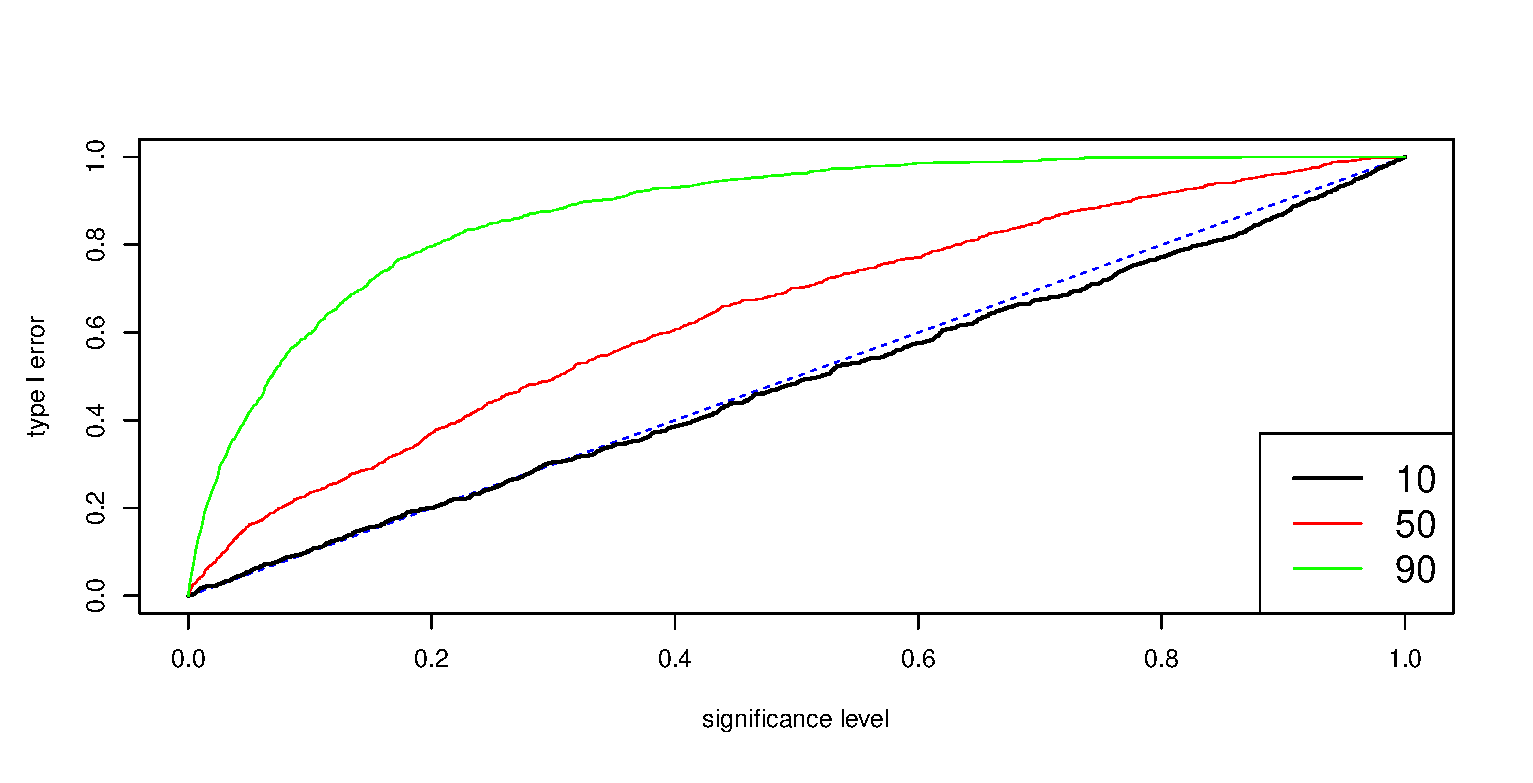
\includegraphics[width=0.65\textwidth]{images/alphaI_phi7_N100.eps}
			\caption{Ошибка первого рода}
		\end{subfigure}\\
		\begin{subfigure}[t]{\textwidth}
			\centering
			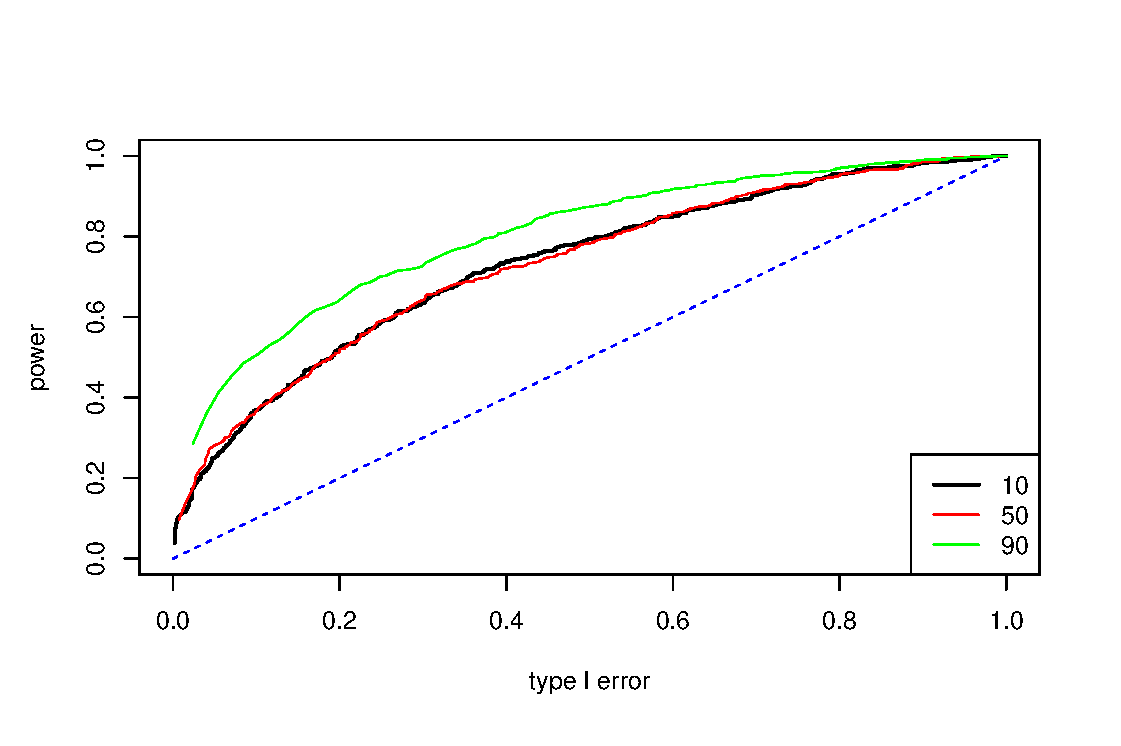
\includegraphics[width=0.65\textwidth]{images/roc_phi7_N100.eps}
			\caption{ROC-кривая ($\omega = 0.075$)}
		\end{subfigure}\hspace{\fill}
		\caption{Пример 1. $\varphi = 0.7$, $N=100$}
	\end{figure}
\end{frame}

\begin{frame}{Пример 2. $\varphi=0.3$, $N=100$}
	\begin{figure}
		\centering
		\begin{subfigure}[t]{\textwidth}
			\centering
			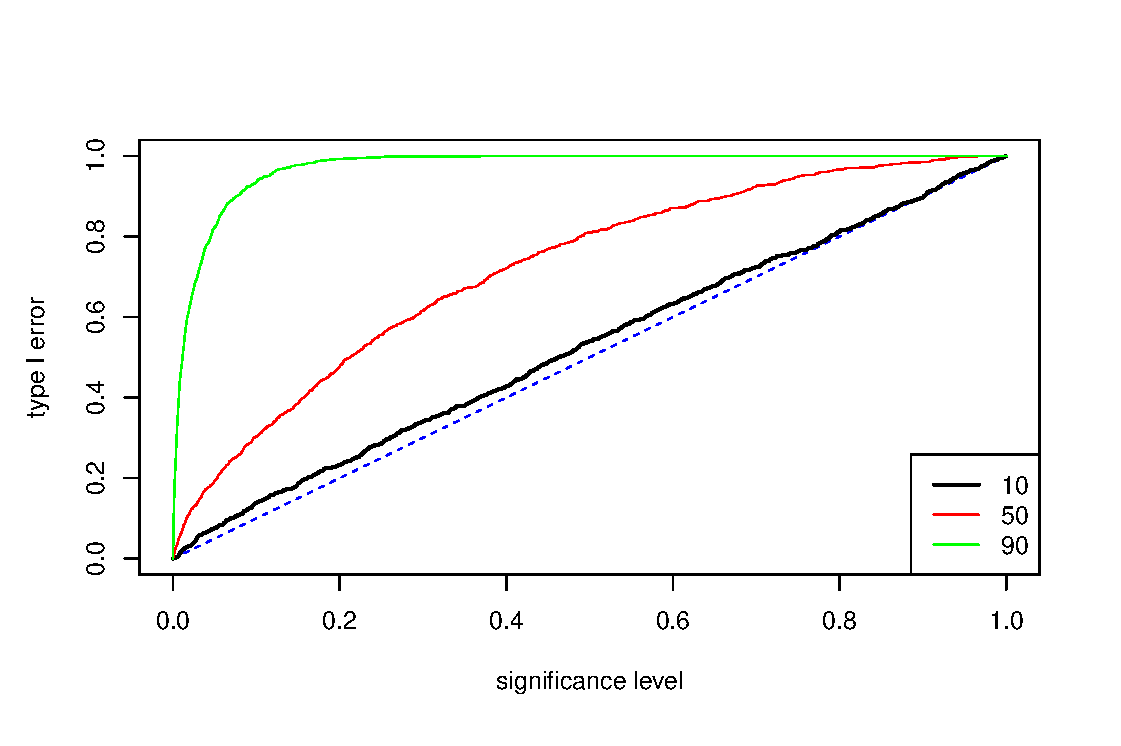
\includegraphics[width=0.65\textwidth]{images/alphaI_phi3_N100.eps}
			\caption{Ошибка первого рода}
		\end{subfigure}\\
		\begin{subfigure}[t]{\textwidth}
			\centering
			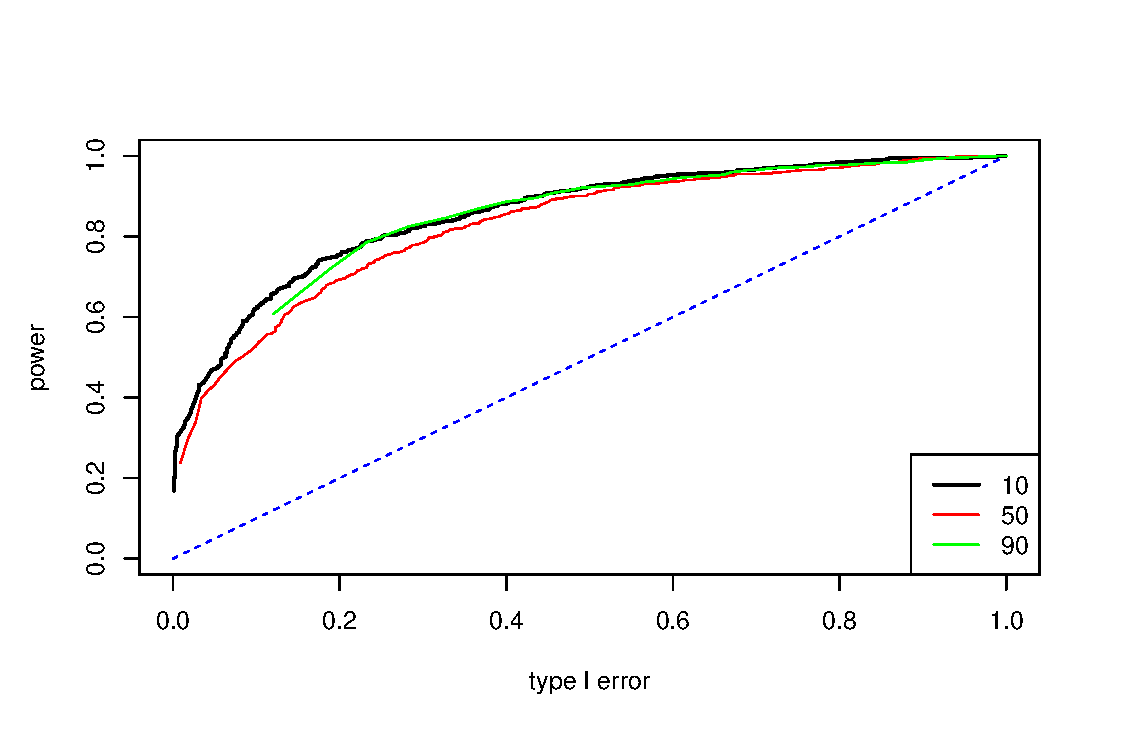
\includegraphics[width=0.65\textwidth]{images/roc_phi3_N100.eps}
			\caption{ROC-кривая ($\omega = 0.075$)}
		\end{subfigure}\hspace{\fill}
		\caption{Пример 2. $\varphi = 0.3$, $N=100$}
	\end{figure}
\end{frame}

\begin{frame}{Пример 3. $N=400$}
	\begin{figure}
		\centering
		\begin{subfigure}[t]{\textwidth}
			\centering
			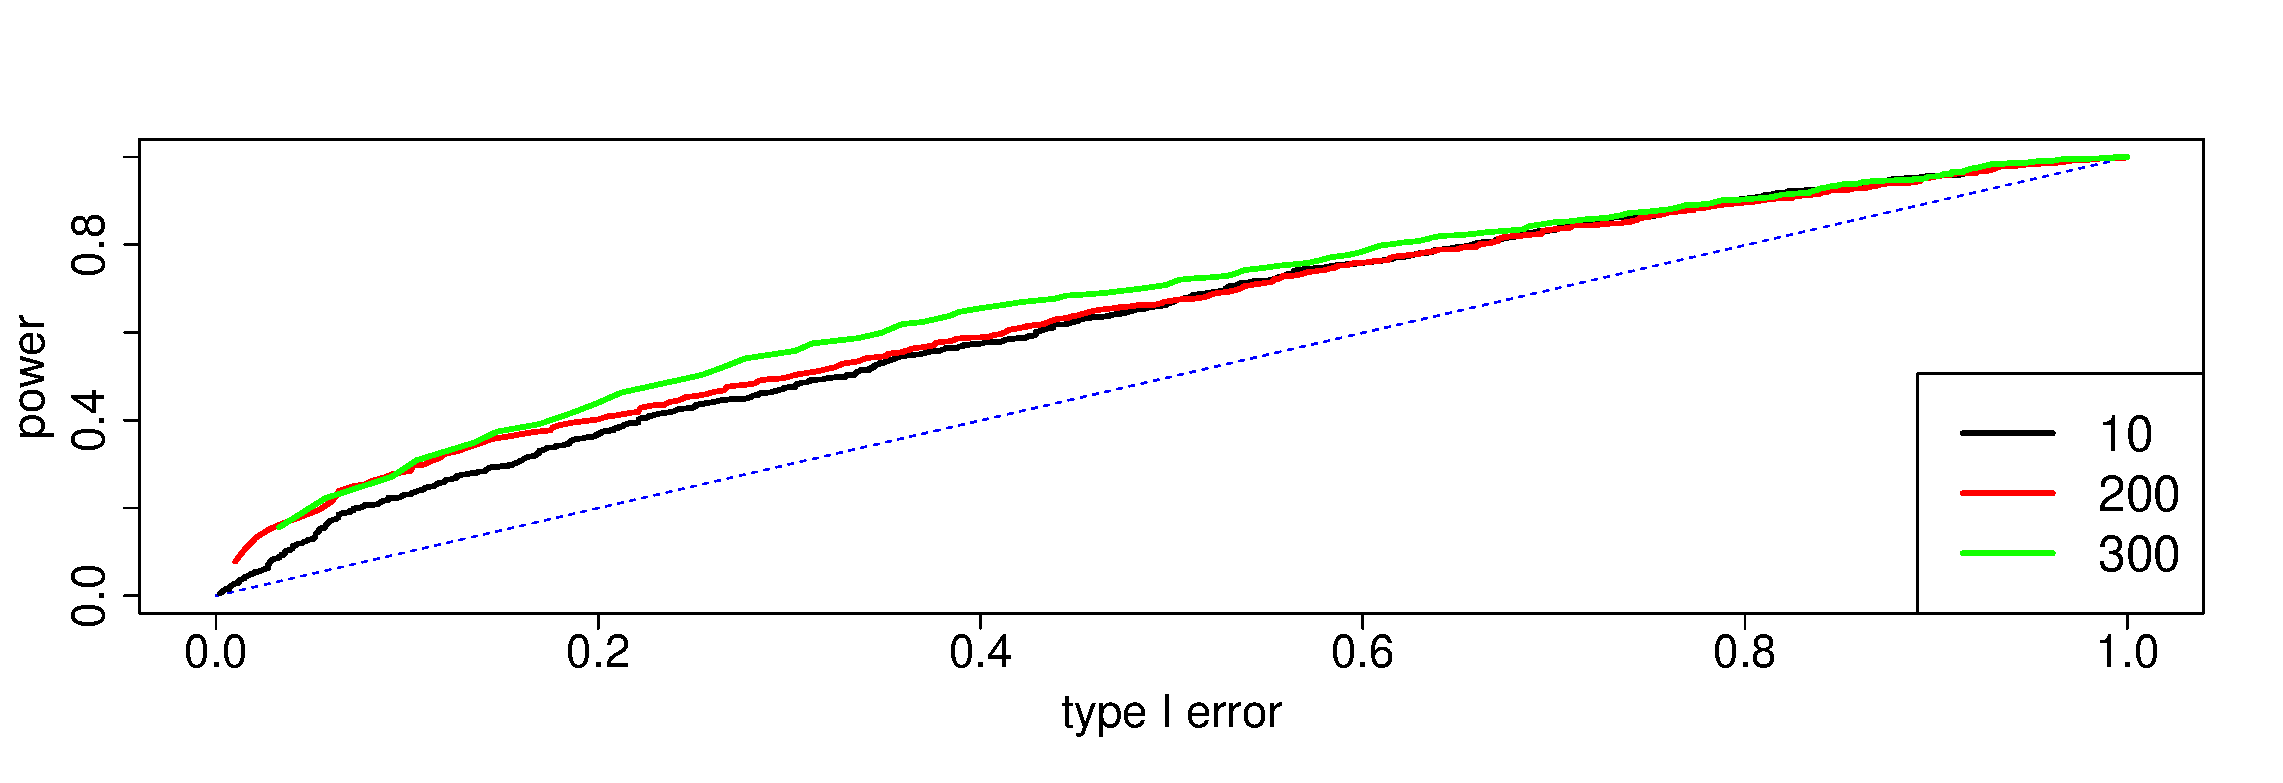
\includegraphics[width=0.65\textwidth]{images/roc_phi7_N400.eps}
			\caption{ROC-кривая ($\varphi = 0.7$, $\omega = 0.075$)}
		\end{subfigure}\\
		\begin{subfigure}[t]{\textwidth}
			\centering
			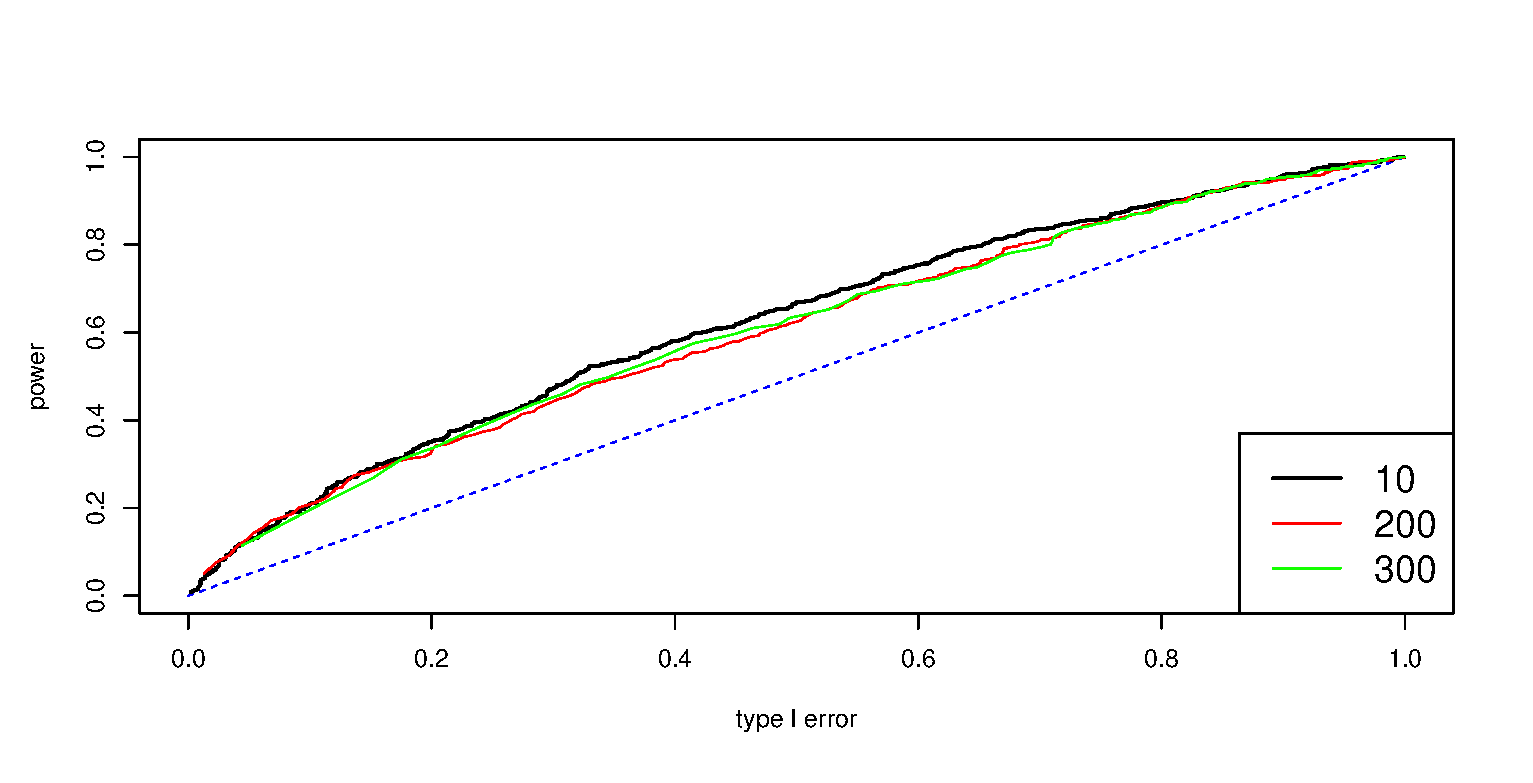
\includegraphics[width=0.65\textwidth]{images/roc_phi3_N400.eps}
			\caption{ROC-кривая ($\varphi = 0.3$, $\omega = 0.075$)}
		\end{subfigure}\hspace{\fill}
		\caption{Пример 3. $N=400$}
	\end{figure}
\end{frame}

\begin{frame}{Пример 4. Зависимость от параметров сигнала}
	\begin{figure}
		\centering
		\begin{subfigure}[t]{\textwidth}
			\centering
			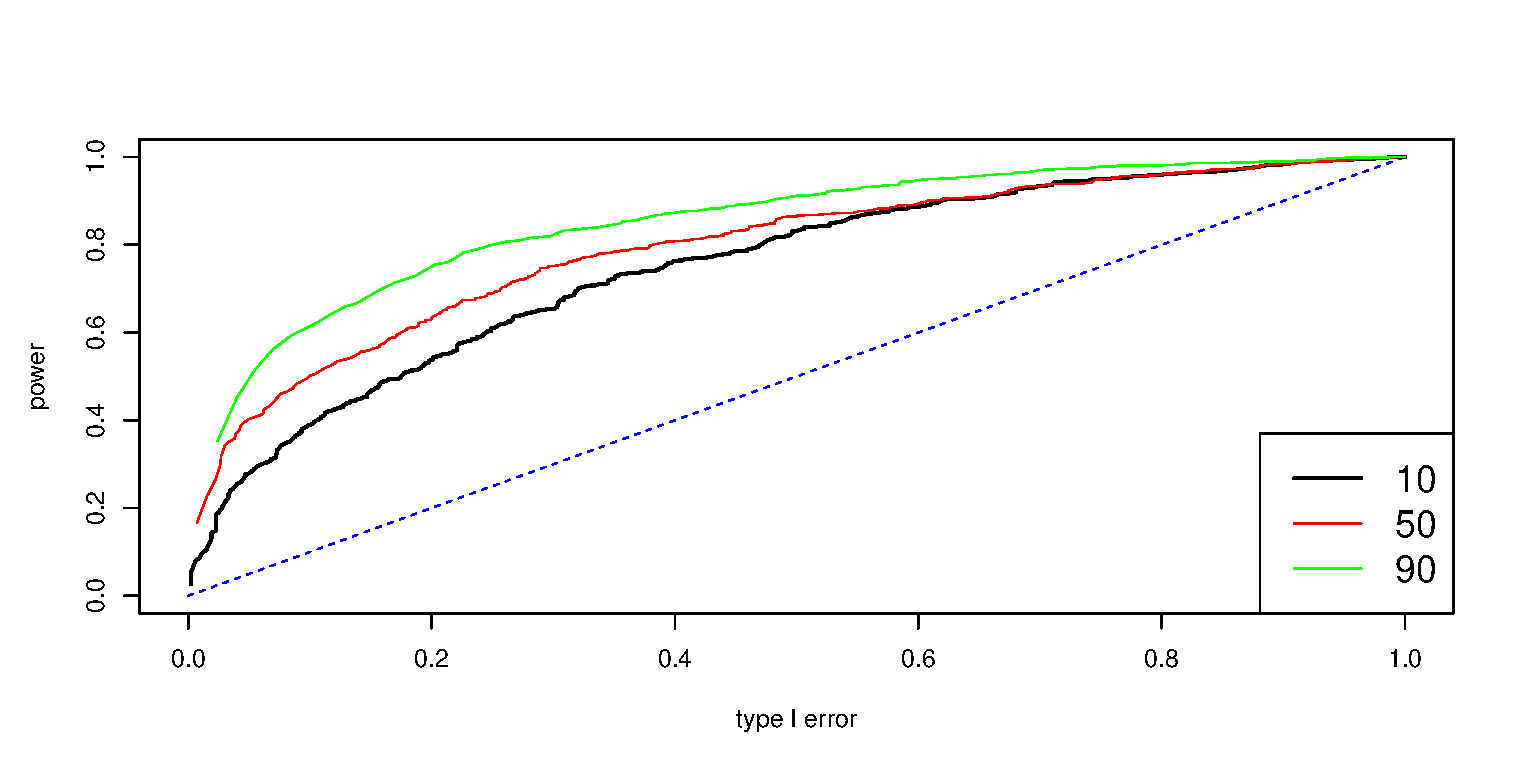
\includegraphics[width=0.65\textwidth]{images/roc_omega0175.eps}
			\caption{ROC-кривая ($\omega = 0.175$)}
		\end{subfigure}\\
		\begin{subfigure}[t]{\textwidth}
			\centering
			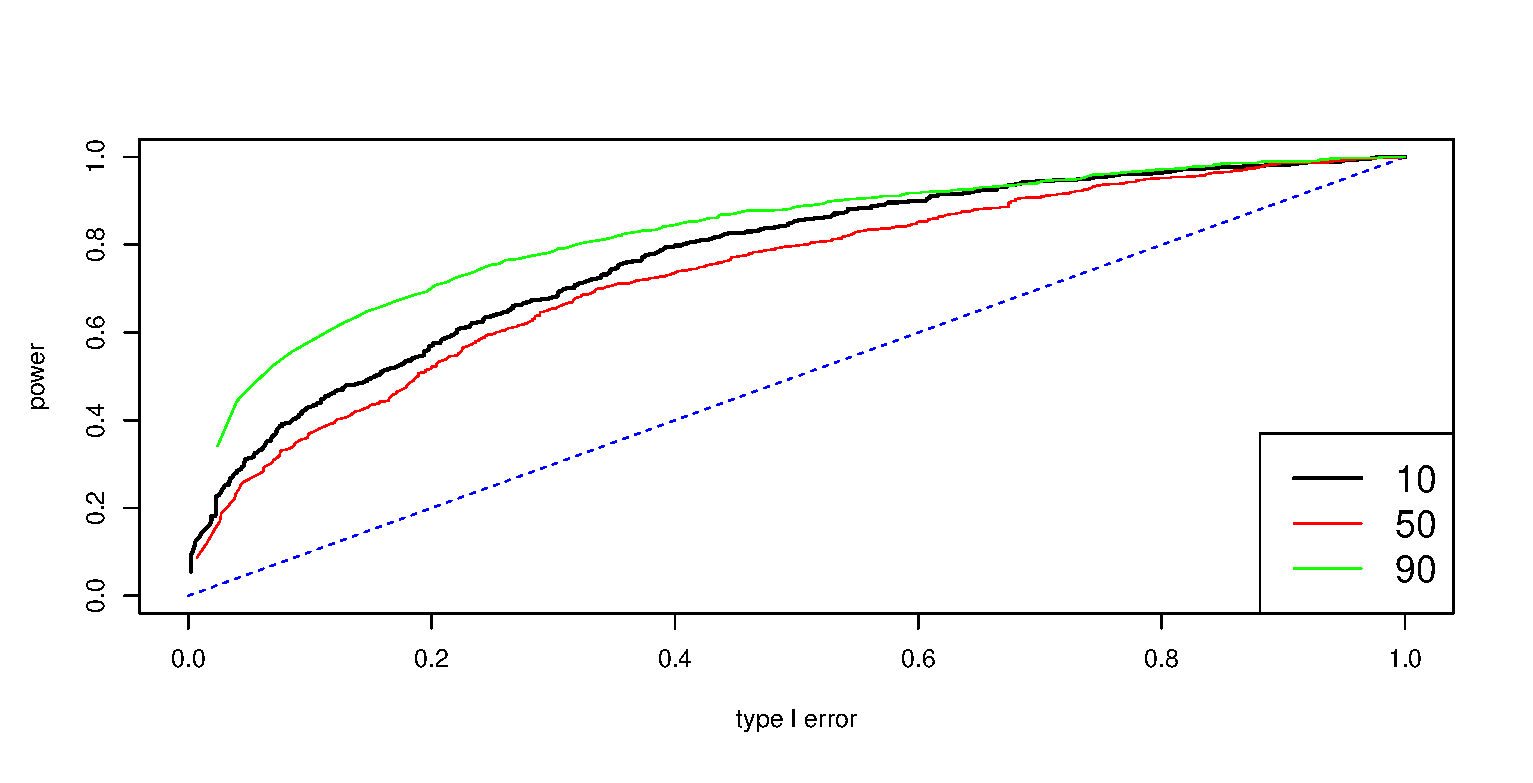
\includegraphics[width=0.65\textwidth]{images/roc_omega0025.eps}
			\caption{ROC-кривая ($\omega = 0.025$)}
		\end{subfigure}

		\caption{Пример 4. $\varphi = 0.7$, $N = 100$}
	\end{figure}
\end{frame}

\begin{frame}{Заключение}
	Численные эксперименты показали, что длина окна $L$, дающая наибольшую мощность, зависит от параметров шума, длины ряда и частоты сигнала в $H_1$.\medskip

	На их основе были выработаны следующие рекомендации:
	\begin{enumerate}
		\item Первый вариант "--- использовать поправленный критерий MC-SSA с $L = 10$. \bluetext{Плюсы}: нетрудозатратно, а также критерий не сильно радикальный. \bluetext{Минус}: такой выбор $L$ может являться неоптимальным, т.е. возможна некоторая потеря в мощности.
		\item Второй вариант "--- построить зависимость оптимальной длины окна от параметров ряда с помощью численного моделирования. Это возможно, если есть дополнительная информация о диапазоне возможных частот в ряде.
	\end{enumerate}
\end{frame}

\end{document}